% HEADERS
%%%%%%%%%%%%%%%%%%%%%%%%%%%%%%%%%%%%%%%%%%%%%%%%%%%%%%%%%%%%%%%%%%%%%%%%%%%%%%%%%%%%%%
\documentclass[11pt,a4paper]{report}
%\usepackage[italian]{babel}
\usepackage{graphicx}
\usepackage{wrapfig}
\usepackage{verbatim}
\usepackage{listings}
\usepackage{xcolor}
\usepackage{hyperref}
\usepackage{float}
\usepackage{titlesec}
\usepackage{nomencl}
\usepackage{amsmath}
\usepackage{epsfig}
\usepackage{wasysym}
\usepackage{gensymb} 
\usepackage{subfig}
\psdraft
\makenomenclature
\usepackage{marginnote}

\renewcommand{\vec}[1]{\mathbf{#1}}
\let\oldhat\hat
\renewcommand{\hat}[1]{\oldhat{\mathbf{#1}}}

\titleformat{\part}[display]
  {\Huge\bfseries}
  {}
  {0pt}
  {}

\titleformat{\chapter}[display]
 {\huge\bfseries}
 {}
 {0pt}
 {}

 \titleformat{\section}[display]
 {\Large\bfseries}
 {}
 {0pt}
 {\thesection\  \ }

\def\UrlBreaks{\do\/\do-}
\hypersetup{
    colorlinks=true,
    linkcolor=black,
    filecolor=magenta,
    urlcolor=cyan,
}
%\usepackage{url}
\definecolor{codegreen}{rgb}{0,0.6,0}
\definecolor{codegray}{rgb}{0.5,0.5,0.5}
\definecolor{codepurple}{rgb}{0.58,0,0.82}
\definecolor{backcolour}{rgb}{0.95,0.95,0.92}

\lstdefinestyle{mystyle}{
    backgroundcolor=\color{backcolour},
    commentstyle=\color{codegreen},
    keywordstyle=\color{magenta},
    numberstyle=\tiny\color{codegray},
    stringstyle=\color{codepurple},
    basicstyle=\ttfamily\footnotesize,
    breakatwhitespace=false,
    breaklines=true,
    captionpos=b,
    keepspaces=true,
    numbers=left,
    numbersep=5pt,
    showspaces=false,
    showstringspaces=false,
    showtabs=false,
    tabsize=2
}

\graphicspath{ {images/} }

\title{Orbital Mechanics Project}

\author{Marwan Alkady\\ Pedro Bossi N\'{u}\~{n}ez \\\ Demartini Davide\\ Iafrate Davide\\}
\date{\today}
%
%%%%%%%%%%%%%%%%%%%%%%%%%%%%%%%%%%%%%%%%%%%%%%%%%%%%%%%%%%%%%%%%%%%%%%%%%%%%%%%%%%%%%%
% ACTUAL DOCUMENT

\begin{document}

% FRONT COVER AND TABLE OF CONTENTS
%%%%%%%%%%%%%%%%%%%%%%%%%%%%%%%%%%%%%%%%%%%%%%%%%%%%%%%%%%%%%%%%%%%%%%%%%%%%%%%%%%%%%%
\begin{titlepage}
	\clearpage\thispagestyle{empty}
	\centering

%	Titles
%	Information about the University

   \centering \includegraphics[scale=0.7]{logo}

   \vspace{0.5cm}

	{\Huge\textbf{Politecnico di Milano} \\
Master of Science in\\ Space Engineering \\
		 \par}
		\vspace{3cm}
	{\Huge{Orbital Mechanics Project}} \\
	%\vspace{1cm}
	%{\large \textbf{xxxxx} \par}
	\vspace{3cm}
	{\huge Group 33\\}
	\vspace{0.4cm}
	{\LARGE Marwan Alkady 88888 - 88888888\\ Pedro Bossi N\'{u}\~{n}ez 887651 - 10561223\\ Davide Demartini 888657 - 10574461\\ Davide Iafrate 967709 - 10800009\\ \par}

%	Set the date
\vspace{1cm}
	{\Large A.Y. 2020-2021 \par}

	\pagebreak

\end{titlepage}

%\maketitle
\nomenclature{$a$}{semi-major axis}
\nomenclature{$e$}{eccentricity}
\nomenclature{$i$}{inclination}
\nomenclature{$\omega$}{periapsis anomaly}
\nomenclature{$\Omega$}{Right ascension of the ascending node}
\nomenclature{$f$}{true anomaly}
\nomenclature{h}{specific angular momentum per unit mass}
\nomenclature{$r$}{radius}
\nomenclature{$AU$}{Astronomical Unit (1.495978707×10^8 km)}
\nomenclature{$\mu_{\oplus}$}{Gravitational Parameter of Earth}
\nomenclature{$\mu_{\astrosun}$}{Gravitational Parameter of the Sun}
\nomenclature{mjd2000}{modified julian date 2000}

\printnomenclature
\tableofcontents

%%%%%%%%%%%%%%%%%%%%%%%%%%%%%%%%%%%%%%%%%%%%%%%%%%%%%%%%%%%%%%%%%%%%%%%%%%%%%%%%%%%%%%
% TEXT
%%%%%%%%%%%%%%%%%%%%%%%%%%%%%%%%%%%%%%%%%%%%%%%%%%%%%%%%%%%%%%%%%%%%%%%%%%%%%%%%%%%%%%
\part{Assignment 1: Interplanetary Explorer Mission}

\chapter{Introduction}
In this chapter, the aim is to design an interplanetary trajectory from Neptune to Mercury with a flyby of Venus. The mission is to be completed between the dates February 1st 2031 and February 1st 2071.\\
Figure 1 a and b – given orbits\\
The design process is composed of  different consecutive steps:\\
\begin{enumerate}
\item Define the time windows for possible transfer phases (departure, gravity assist and arrival);
\item Set known parameters and compute the orbits of the three planets of interest;
\item Set and solve the Lambert’s problem between first Neptune and Venus and then Venus and Mercury at different times inside the possible time windows;
\item Evaluate the powered gravity assist for every trajectory previously computed;
\item Selection of the most efficient transfer strategy.
\end{enumerate}

\section{Method of patched conics}
The movement of a body inside the interplanetary space cannot be described by the two-body problem since the body itself is subject to the influence of different celestial bodies at once.
In order to study such movement, an approximation is introduced with the method of the patched conics. With this approximation, the influence of a planet or a gas giant is limited to a sphere named Sphere of Influence (SOI from now on) which radius is calculate using the following equation:

\begin{equation*}
    R_{SOI} = R_{CB}\left(\frac{m_{CB}}{m_{\astrosun}}\right)^{\frac{2}{5}}
\end{equation*}

Where $R_{CB}$ is the distance between the celestial body and the sun, $m_{CB}$ is the mass of the central body and $m_{\astrosun}$ is the mass of the sun.\\ 
If the body is outside any planet’s or gas giant’s SOI, then it is considered to be subject only to the Sun’s gravity attraction.\\
Figure 2 – patched conics\\
In this report, the spacecraft is considered to be already outside of Neptune’s SOI at departure and it does not enter Mercury’s SOI at arrival. The spacecraft only enters Venus’ SOI during the flyby.
% table with:
% Departure Planet
% flyby planet
% arrival planet
% minimum departure and maximum arrival dates

\chapter{Mission analysis}

\section{Design process}
\subsection{Time windows}
The Lambert’s problem solution is a section of an elliptical orbit. Furthermore, the minimum time needed to complete a transfer strategy is the time required to run across an elliptical orbit with eccentricity $e\rightarrow1$.

Therefore, given the parabolic times of flight from Neptune to Venus and from Venus to Mercury, it is possible to define the earliest possible date of flyby and arrival starting from the departure date. In particular the earliest possible flyby  and arrival dates can be defined as follows:

\begin{equation*}
    Fly_{min}=Dep_{min}+ ToF_{NV}
\end{equation*}

\begin{equation*}
    Arr_{min}=Fly_{min}+ ToF_{VM}
\end{equation*}

\begin{equation*}
    Fly_{max}=Arr_{max}+ ToF_{VM}
\end{equation*}

Where $ToF_{ij}$ is the parabolic time of flight between the planets i and j.
Similarly, given the latest arrival date it is possible to define the latest flyby and departure dates:

Figure 3 – time windows\\
Said dates are computed using the timeWindows script and they are:

\begin{equation*}
    Dep_{max}=Fly_{max}+ ToF_{NV}
\end{equation*}

\begin{table}[H]
\centering
\begin{tabular}{|l|l|}
\hline
$Fly_{min}$ & 20-04-2043 \\ \hline
$Arr_{min}$ & 28-04-2043 \\ \hline
$Dep_{max}$ & 06-11-2058 \\ \hline
$Fly_{max}$ & 23-01-2071 \\ \hline
\end{tabular}
\end{table}



\subsection{Additional constraints considered}
One additional constraint that was to be considered is the minimum altitude of the perigee point for the planetocentric hyperbola. We chose this as 200 km, giving us a minimum radius of perigee ofCHECCKKK 6350km++++. For the MATLAB fmincon optimization function this was set using an additional constraint function and also time constraints based on the parabolic time of flights were set using the inequality matrices.

\subsection{Transfer options exploration, analysis and comparison}
For the selection of an optimum transfer we employed different strategies together.
To analyze the solutions we built an objective function giving us the $\Delta V$ needed for the transfer given the \emph{arrival}, \emph{gravity assist} and \emph{departure} dates inserted to the function. The function computes the two arcs connecting planets at departure and flyby and the flyby planet to the arrival planet. The outputs consist of the total $\Delta V$ required, then the $\Delta V$'s for the separate legs and the informations for each transfer arc as an object with various properties useful for the rest of the analysis and plotting.

\lstset{style=mystyle}
\begin{lstlisting}[frame=single,caption=GAtransfer objective function structure]  
compute first arc
compute second arc
join them with flyby
output total DV 
\end{lstlisting}


\subsubsection{Coarse grid search}
The first step is a coarse grid search using three nested for loops:\\

\lstset{style=mystyle}
\lstinputlisting[language=Matlab,caption=coarse grid search,linerange={64-88}]{InterplanetaryMission_group_33.m}

\subsubsection{fmincon refinement}
The objective function GAtransfer can also be used for the fmincon MATLAB optimization function, which finds the minimum for a constrained nonlinear function using a gradient-based optimizer. This function takes as initial guess the minimum point found from the coarse grid search as a vector of 3 mjd2000 dates, the linear constraint on the window with two $\vec{ub}$ and $\vec{lb}$ vectors, the time of flight constraints with the $\vec{A}$ and $\vec{b}$ inequality matrices and the \emph{nonlinear constraint} on the minimum radius of the hyperbola as a function flyby\_CONSTR\\
\subsubsection{Other strategies explored}

We also explored using the \emph{genetic algorithm} ("ga" MATLAB function) to find an initial guess to then refine further using fmincon; however due to heuristic algorithm this gave us worse and often inconsistent results between successisve runs of the program.

\subsection{Selection of the final solution}
The final solution was selected as the one given from the coarse grid search plus the fmincon refinement as this gave us a lower total $\Delta V$. By narrowing the windows we also found other shorter transfers but with an higher total $\Delta V$ so we decided to discard them.
% with plots and stuff

\section{Final solution}

\subsection{Heliocentric trajectory}
The final transfer strategy is composed of four arcs: the first and the last one lie inside the Sun’s SOI; the second and third one are inside Venus’ SOI (and are analyzed in a later paragraph). 
The Transfer strategy is completed between the times 02:54:32 on June 27th 2032 and 03:09:55 on July 11th 2070. The powered flyby is performed at 13:49:55 on July 11th 2061.\\
Figure - complete strategy\\
The first arc connects Neptune and Venus orbits. It is characterised by the following data:

\begin{table}[H]
\centering
\resizebox{\textwidth}{!}{%
\begin{tabular}{|c|c|c|c|c|}
\hline
\textbf{a [AU]} & \textbf{e [-]} & \textbf{i [°]} & \textbf{RAAN [°]} & \textbf{$\omega$  [°]} \\ \hline
15,1835         & 0,9487         & 1,5798         & 109,6640          & 85,2838                \\ \hline
\end{tabular}%
}
\end{table}

The initial position is characterised by a true anomaly (f) of 180,2552°. In Cartesian coordinates the initial point is identified by the following data:

\begin{table}[H]
\centering
\resizebox{0.75\textwidth}{!}{%
\begin{tabular}{|c|c|c|}
\hline
\textbf{R$_x$ [AU]}   & \textbf{R$_y$ [AU]}   & \textbf{R$_z$ [AU]}   \\ \hline
28.8260   & 7.8326    & -0.8213   \\ \hline
\textbf{v$_x$ [km/s]} & \textbf{v$_y$ [km/s]} & \textbf{v$_z$ [km/s]} \\ \hline
-0.3810               & 0.8955               & 0.0016               \\ \hline
\end{tabular}%
}
\end{table}

The initial position’s distance from the Sun is 29,8825AU and the velocity at the initial point is 0,9732 km/s.
The final position is characterized by a true anomaly (f) of 94,7162°. In Cartesian coordinates the initial point is identified by the following data:

\begin{table}[H]
\centering
\resizebox{0.75\textwidth}{!}{%
\begin{tabular}{|c|c|c|}
\hline
\textbf{R$_x$ [AU]}   & \textbf{R$_y$ [AU]}   & \textbf{R$_z$ [AU]}   \\ \hline
0.3421   & -0.9573   & 0  \\ \hline
\textbf{v$_x$ [km/s]} & \textbf{v$_y$ [km/s]} & \textbf{v$_z$ [km/s]} \\ \hline
36.6802              & -18.4610              & -0.7813              \\ \hline
\end{tabular}%
}
\end{table}

The initial position’s distance from the Sun is 1,0166 AU and the velocity at the initial point is 41,0714 km/s.
The fourth arc connects the point where the spacecraft exits the Venus’ sphere of influence with Mercury.

% Departure, flyby and arrival times.
% Plot of the heliocentric trajectory,together with the orbits of
% the three planets and their positions at departure, flyby and arrival.

\subsection{Powered gravity assist}
% Altitude of the closest approach.
% Time duration of the flyby (considering a finite SOI).
% Compare total flyby \Delta v with the cost of the manoeuvre \Delta v_{ga}
% Plot of the incoming and outcoming hyperbola arcs

\subsection{Cost of the mission}
%\Delta v_{dep}, \Delta v_{ga}, \Delta v_{arr}.

\part{Assignment 2: Planetary Explorer Mission}

\chapter{Mission requirements}
In this chapter we are going to explain how we have designed a planetary explorer
mission to perform Earth observation: we were in fact required to analyse the Earth-centred orbit characterised by the values in the table below and estimate its ground track, studying the effects of the assigned orbit perturbations by integrating both Gauß’s planetary equations and Cartesian equations and subsequently comparing the results of the two methods. After the characterisation of the ground track, we propose a modification of the orbit aimed to get a ground track which repeats itself once a sidereal day.\\

\begin{table}[H]
\centering
\resizebox{\textwidth}{!}{%
\begin{tabular}{|c|c|c|c|}
\hline
\textbf{a} [$10^4 km$]                                                       & \textbf{e}             & \textbf{i} [deg]   & \textbf{hp} [km]             \\ \hline
4.0718                                                            & 0.6177        & 78.2195   & 15566.491           \\ \hline
\begin{tabular}[c]{@{}c@{}}\textbf{Repeating GT} \\ \textbf{ratio k:m$^{note}$}\end{tabular} & \textbf{Perturbations} & \multicolumn{2}{c|}{\textbf{Parameters}} \\ \hline
1:1                                                               & J2 and SRP    & cR = 1.2  & A/m = 4.000 $m^2/kg$  \\ \hline
\end{tabular}%
}
\caption{Mission requirements}
\label{tab:Mission_requirements}
\end{table}

\marginnote{\textbf{Note}: the grountrack repeats itself \textbf{k} times every \textbf{m} revolutions of the planet.}[-4cm]

\chapter{Mission analysis outputs}

\section{Nominal orbit}
%initial values and main characteristics

\section{Ground track}
% GT considering only J2 as perturbation and GT considering the assigned perturbation
\begin{figure}[H]
\centering
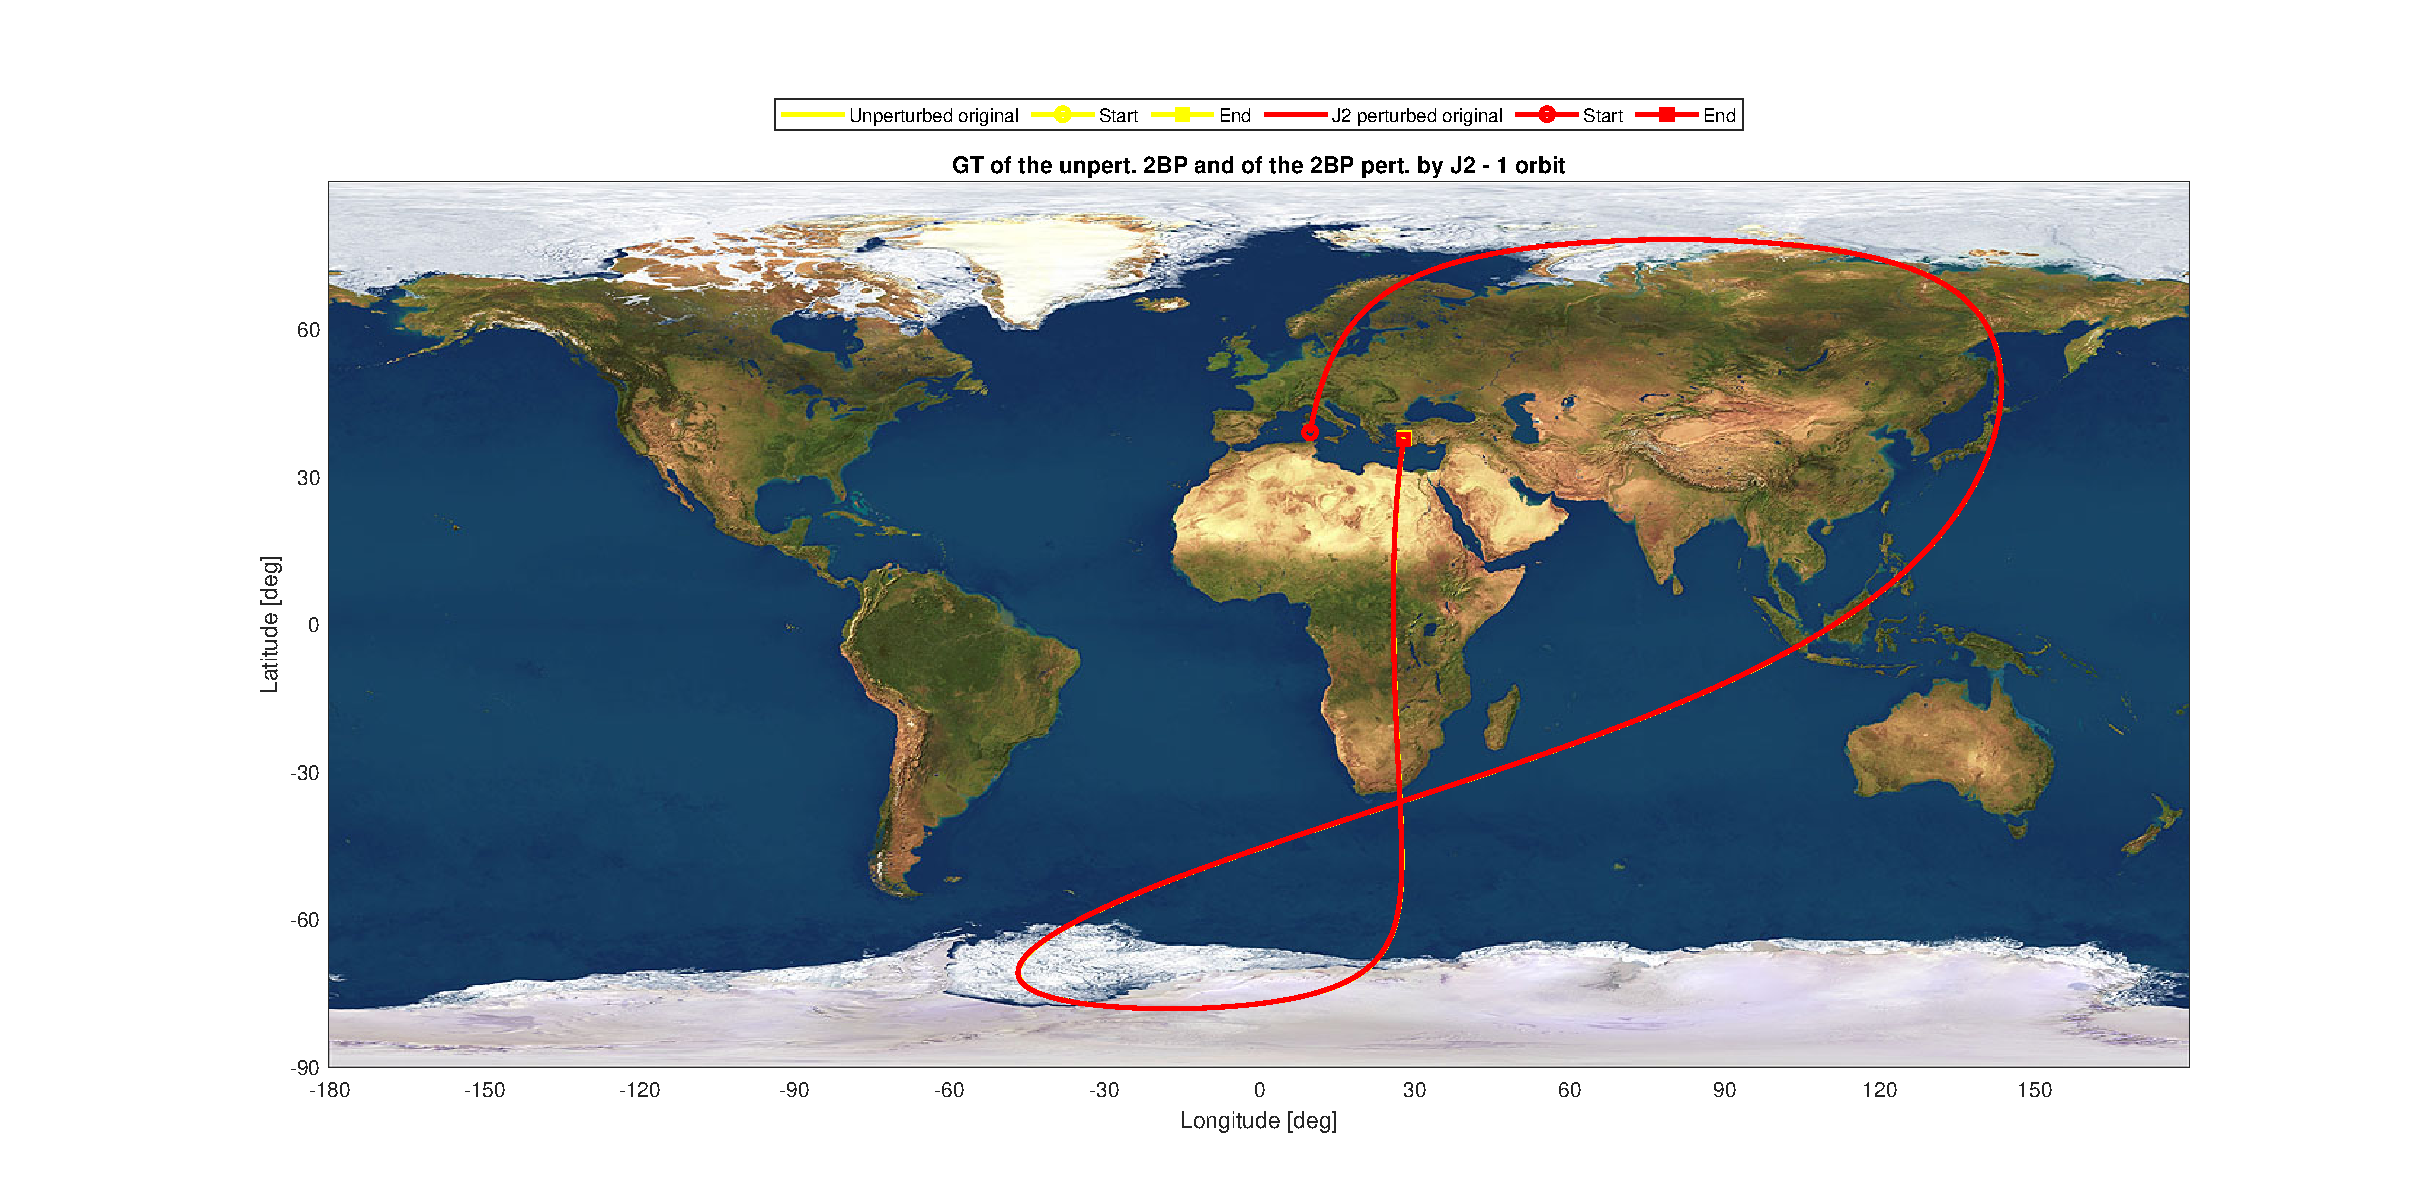
\epsfig{file=oneperiod.eps, width=1\textwidth}
\end{figure}
\begin{figure}[H]
\centering
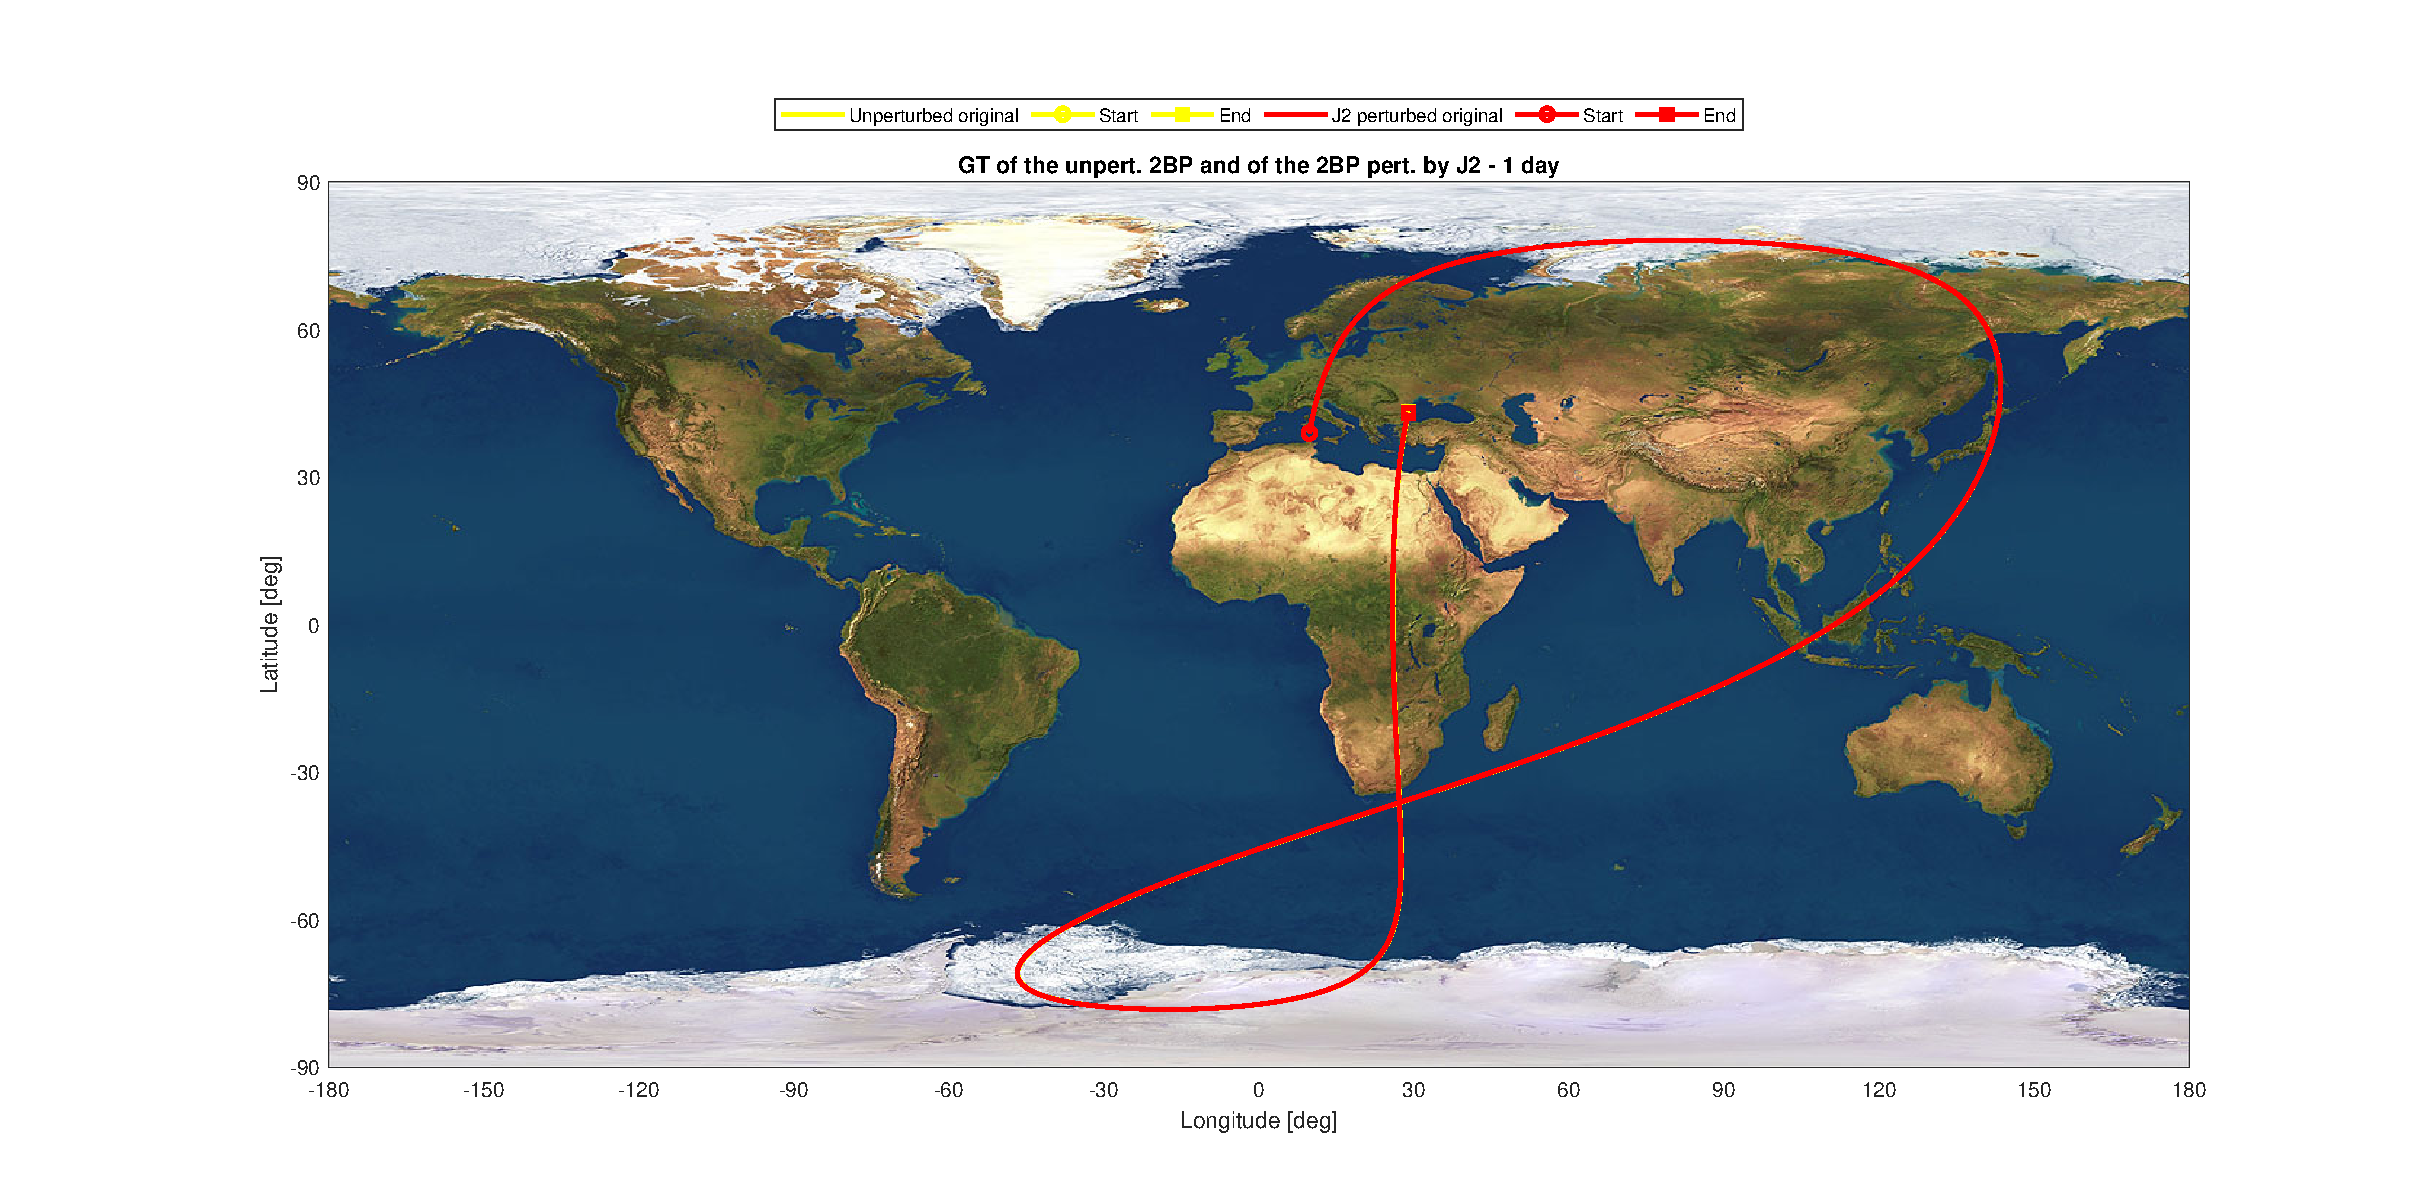
\epsfig{file=oneday.eps, width=1\textwidth}
\end{figure}
\begin{figure}[H]
\centering
\epsfig{file=tendays.eps, width=1\textwidth}
\end{figure}
\begin{figure}[H]
\centering
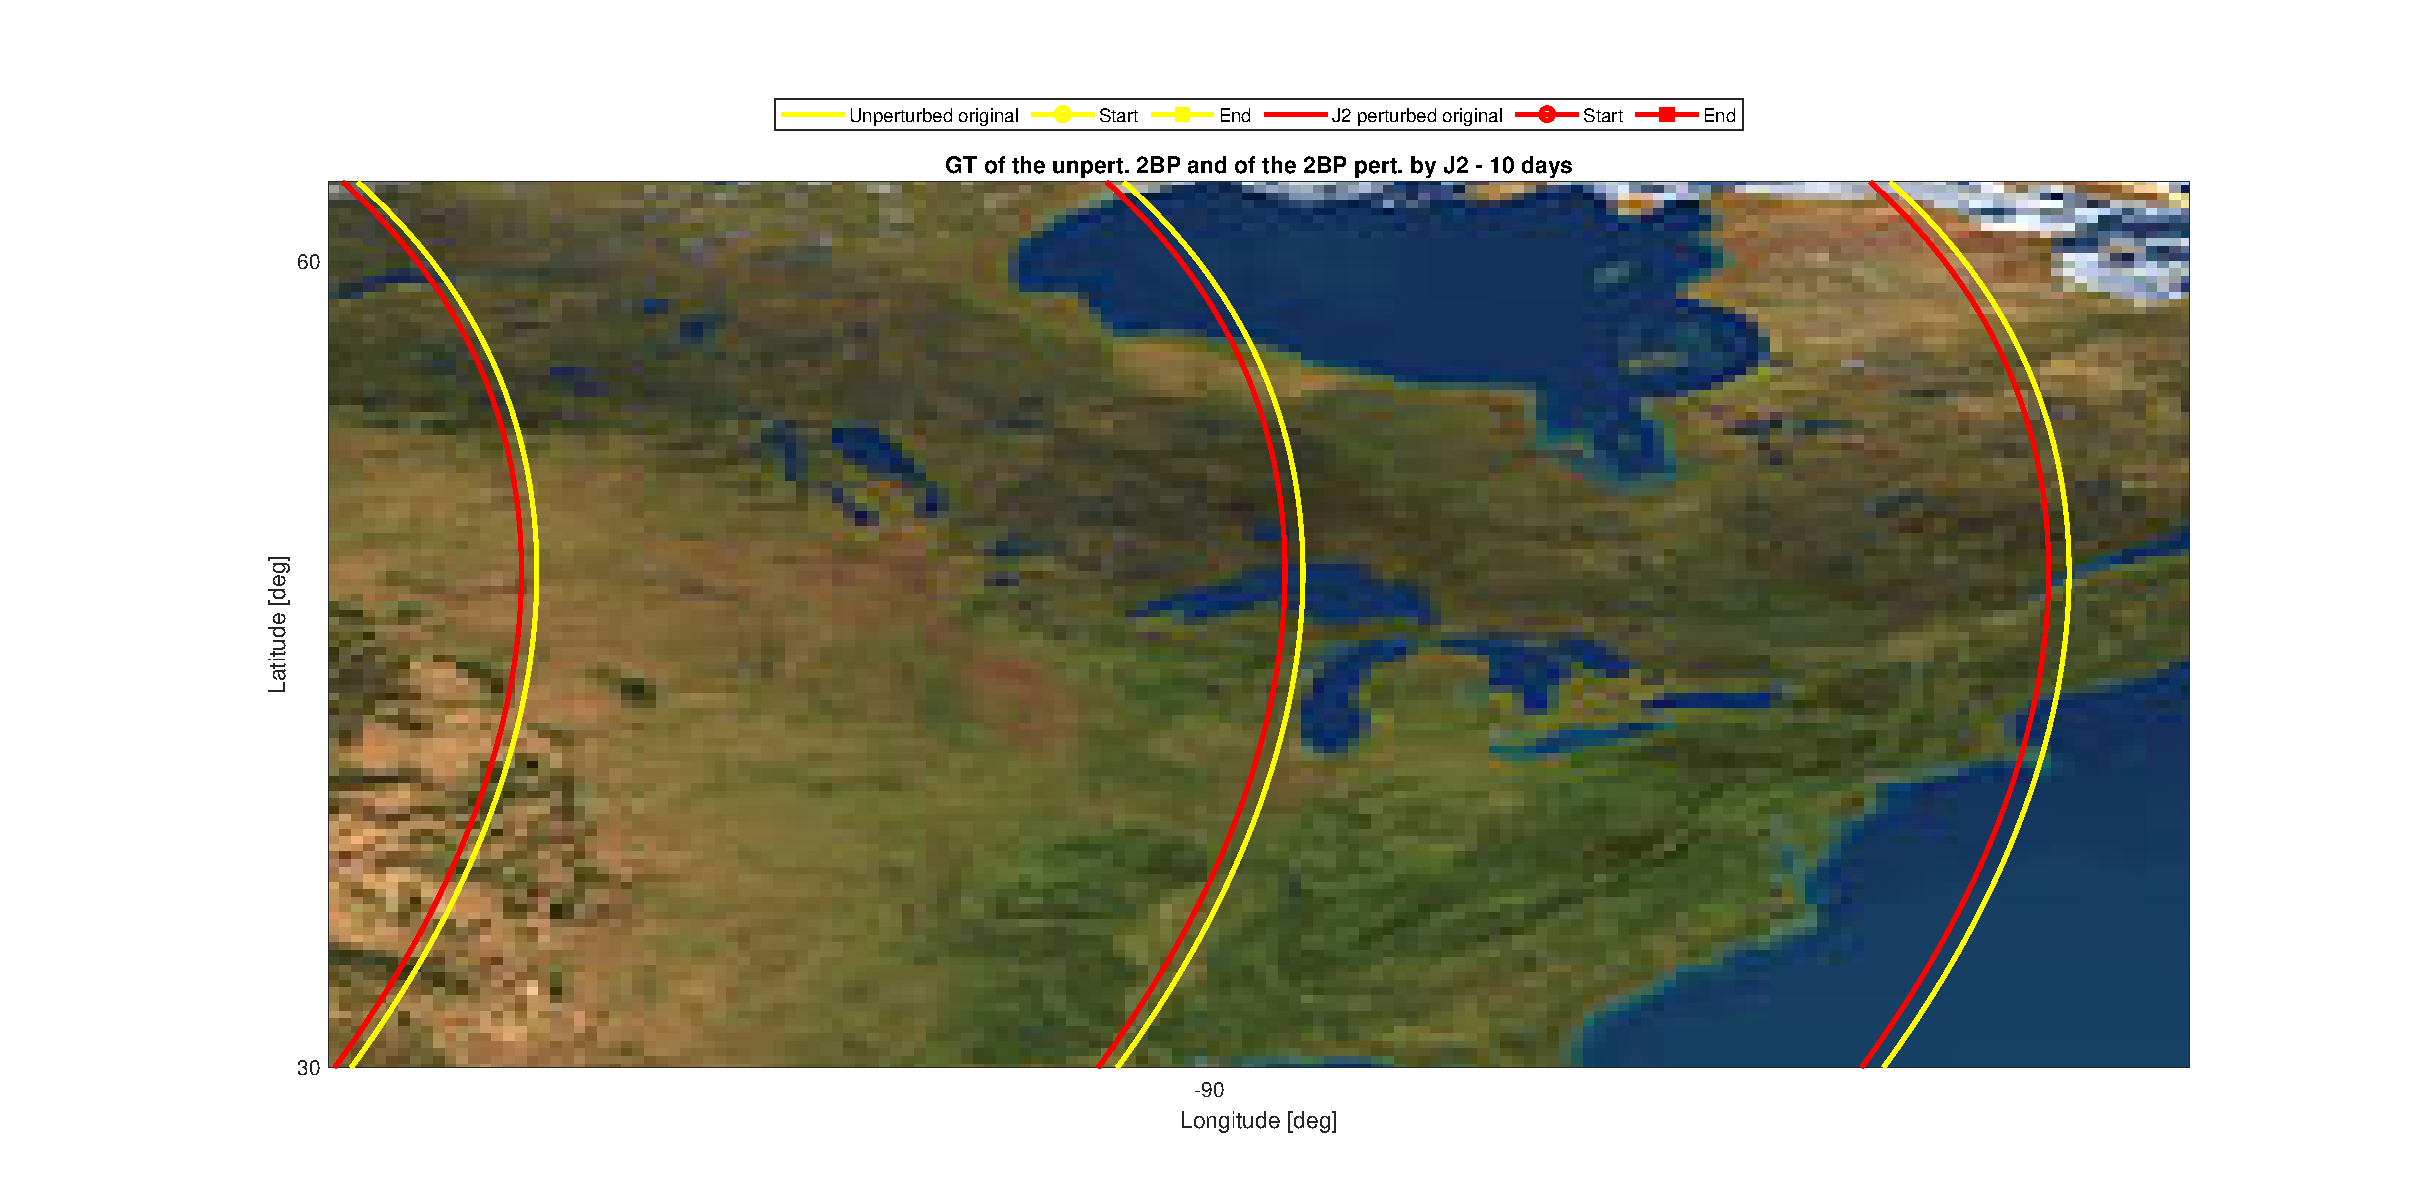
\epsfig{file=tendayscloseup.eps, width=1\textwidth}
\end{figure}
\begin{figure}[H]
\centering
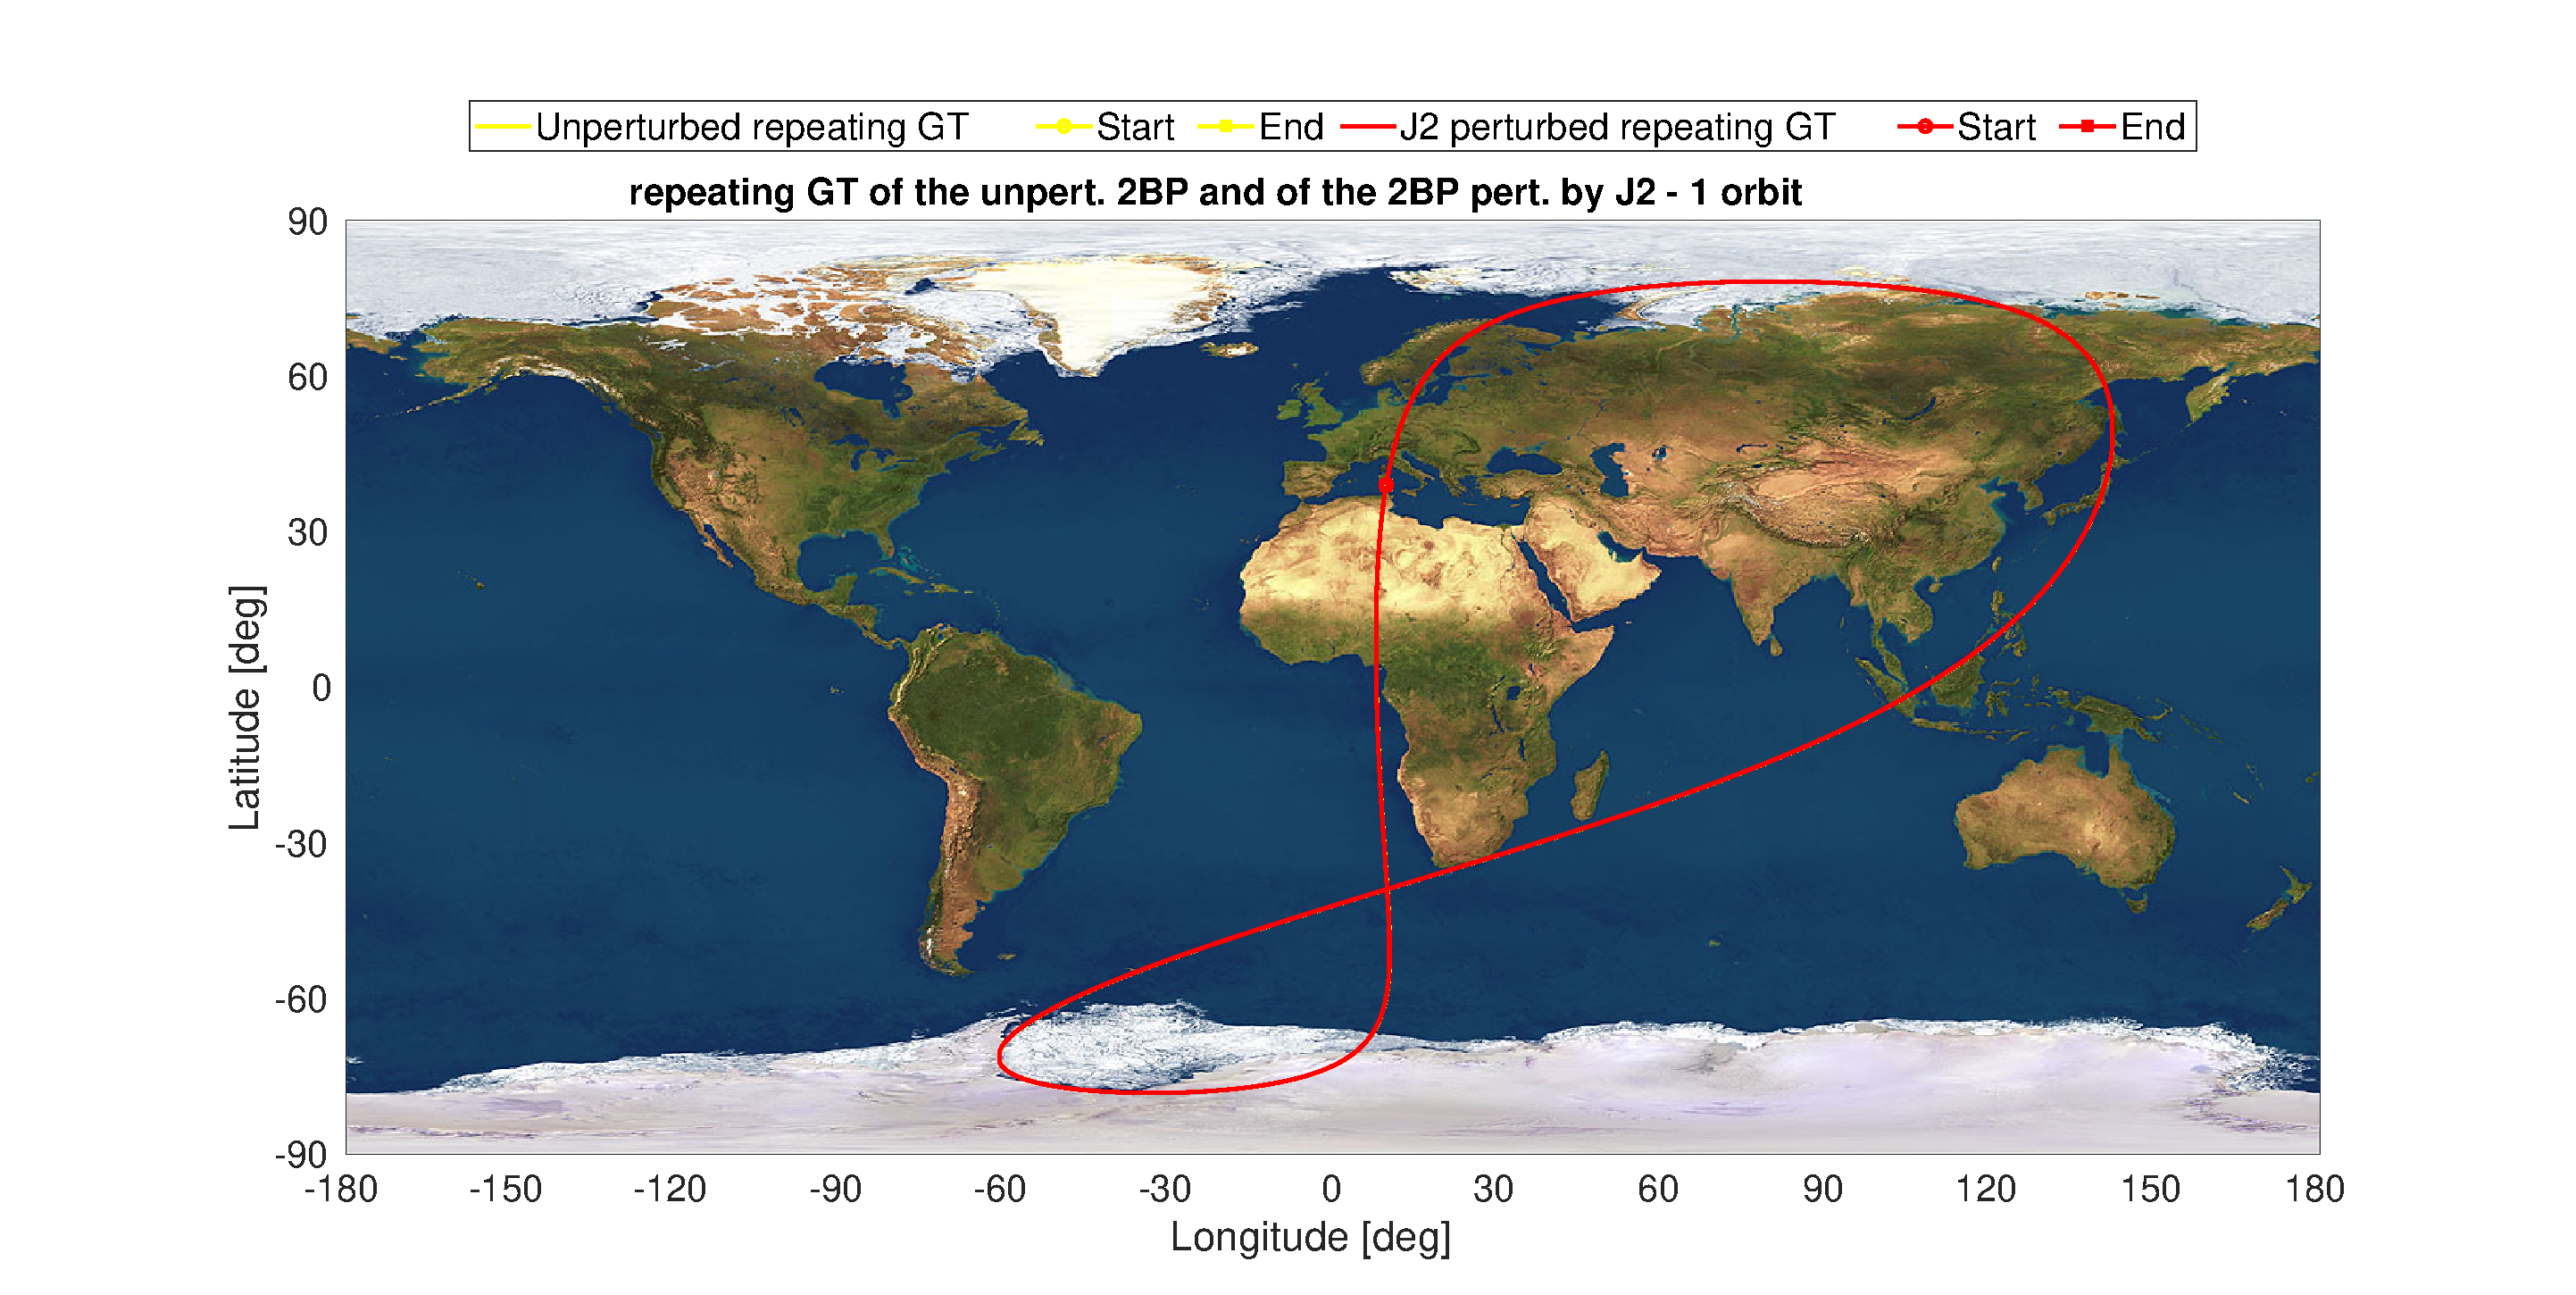
\epsfig{file=repeating.eps, width=1\textwidth}
\end{figure}
\begin{figure}[H]
\centering
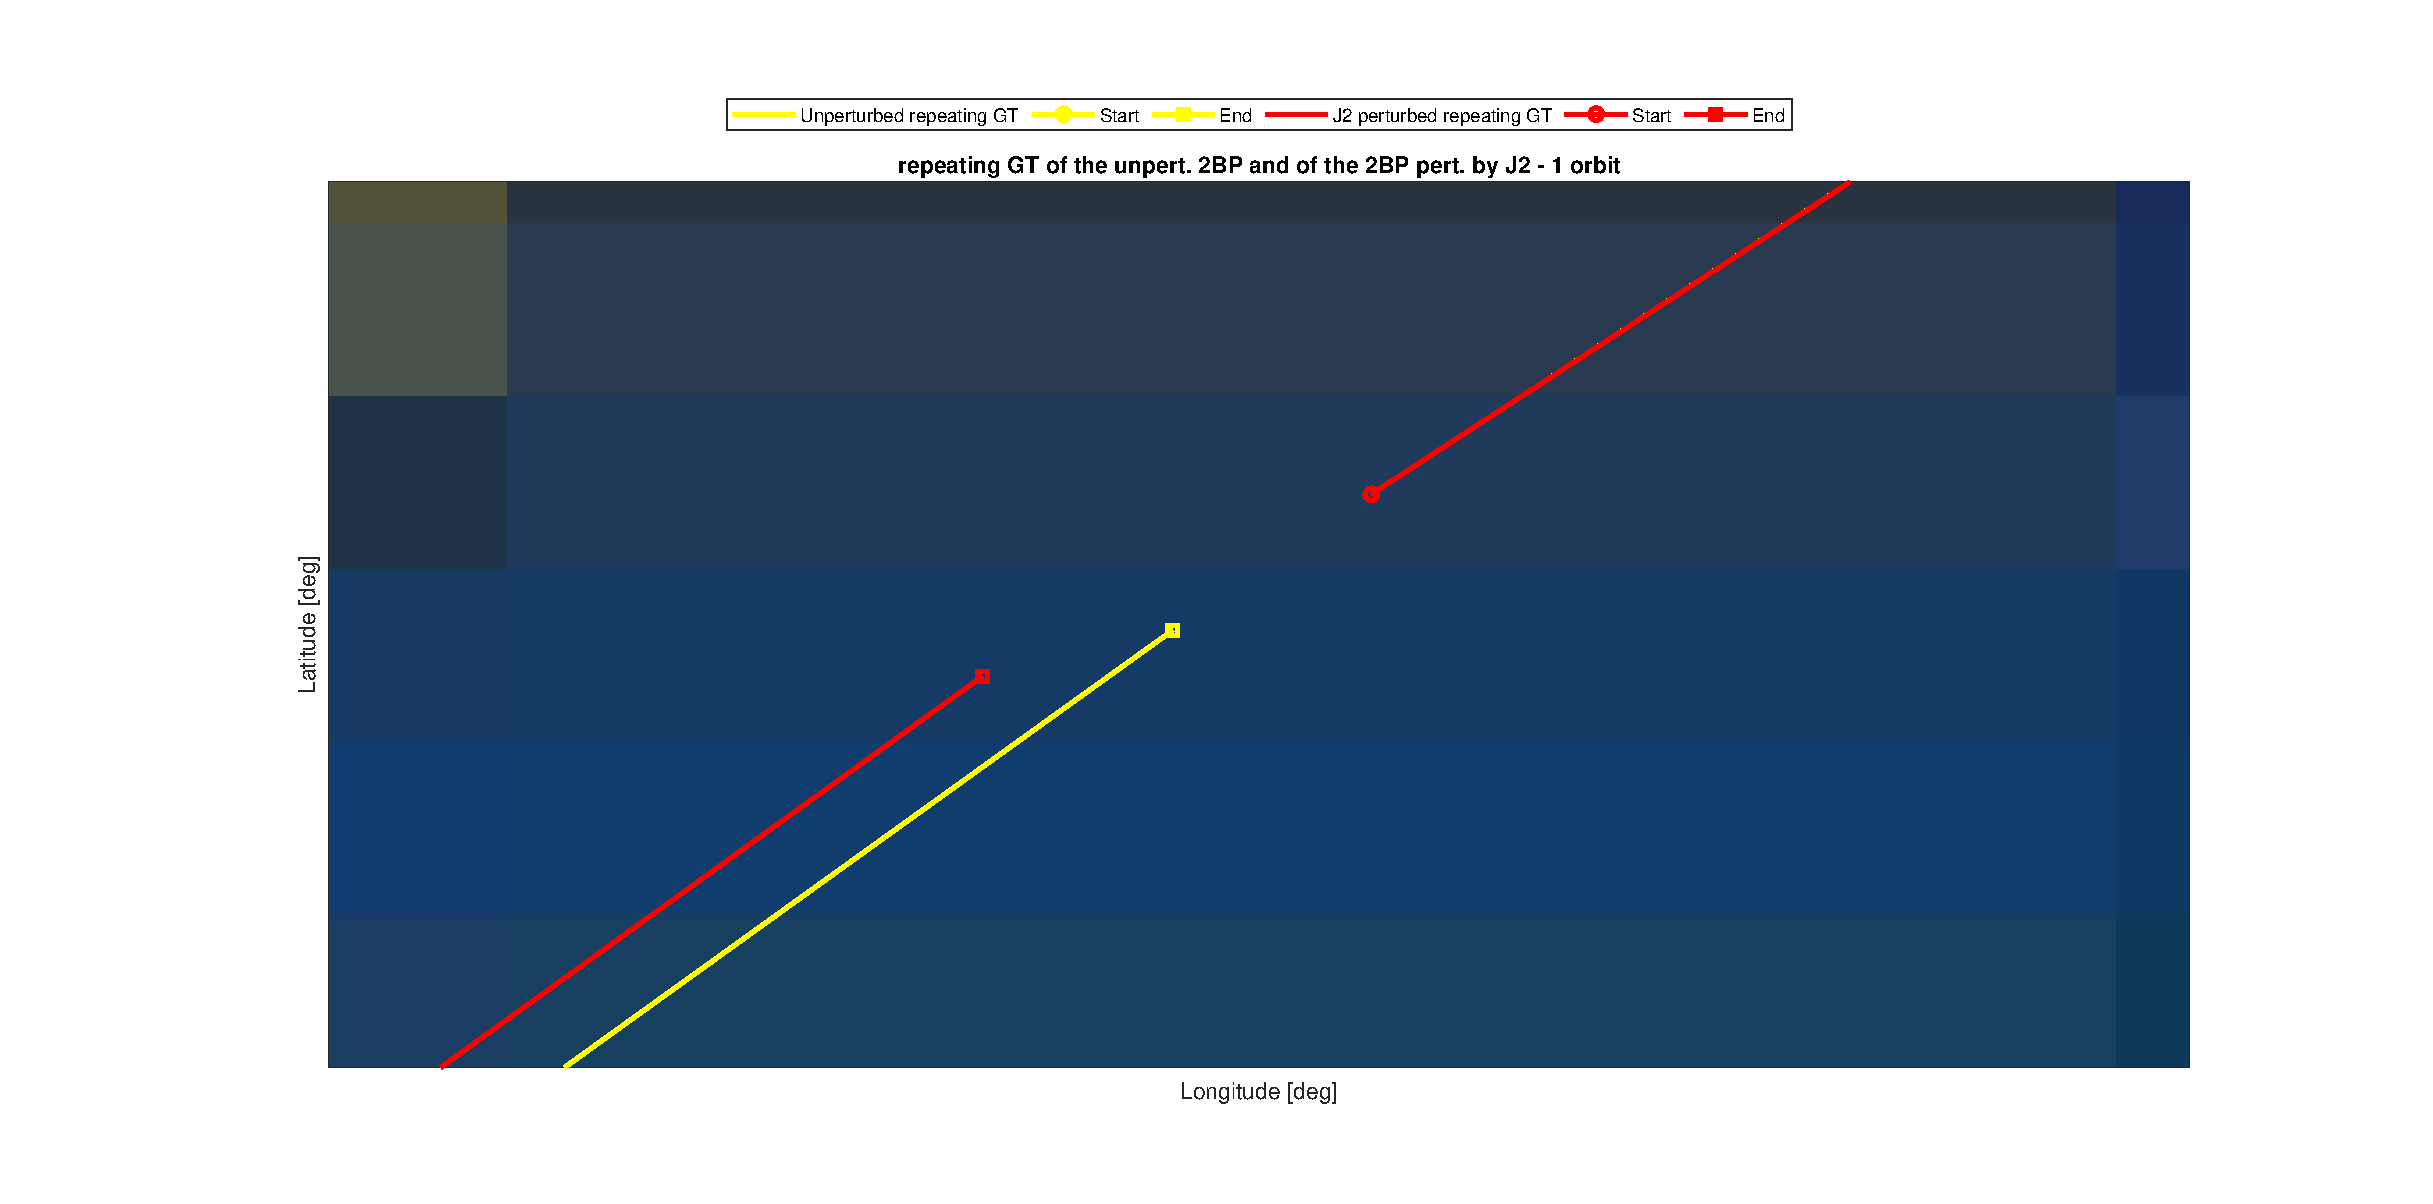
\epsfig{file=repeatingcloseup.eps, width=1\textwidth}
\end{figure}

\section{Orbit Perturbations}
In our model we included perturbations due to two effects:
\begin{itemize}
    \item \textbf{Second Zonal Harmonic \emph{J2}} \par Models the Earth Oblateness using the spherical geopotentials model, truncated to the second term.
    \item \textbf{Solar Radiation Pressure \emph{SRP}} \par A force given by the impact of momentum-carrying photons on the surfaces of the spacecraft. For this perturbation we have written a function that, based on the initial date gets the position vector of the Earth from the ephemerides function and uses that together with the position vector of the spacecraft with respect to the Earth to calculate the direction of the disturbing acceleration. A simple algorithm for the eclipse condition found in \cite{SRP_Curtis} has been implemented.
    \begin{equation}
        \vec{a_{SRP}} = -P_{SR@1AU}\frac{AU^2}{||\vec{r}_{sc-Sun}||^3}c_R\frac{A_{Sun}}{m}\vec{r}_{sc-Sun}
    \end{equation}
\end{itemize}

These forces give an acceleration to the spacecraft so that the total acceleration it perceives in orbit is
\begin{equation}
    \vec{a} = - \frac{\mu_{\oplus}}{r^3}\vec{r} + \vec{a}_{SRP} + \vec{a}_{J2}
\end{equation}

\section{Orbit Propagation}
\subsection{Methods}
% In Cartesian coordinates and Keplerian elements through Gauss’ planetary equations,
%comparison of the propagation methods in terms of accuracy, computational time etc.
To propagate the orbit we used two different methods:
\begin{itemize}
    \item \textbf{Gauss Planetary Equations}
    \par
    \begin{align*}
        \frac{da}{dt}&=\frac{2a^2}{h}\Big(e\sin f \: a_r +\frac{p}{r}a_s\Big)\\
        \frac{de}{dt}&=\frac{1}{h}\Big(p\sin(f) \: a_r+ \Big( (p+r)\cos f +re \Big) a_s\Big)\\
        \frac{di}{dt} &= \frac{r\cos(f+\omega)}{h}a_w\\
        \frac{d\Omega}{dt}&=\frac{r\sin (f+\omega) }{h \sin i}a_w\\
        \frac{d\omega}{dt}&=\frac{1}{he} \Big( \cos f \; a_r + (p+r)\sin f \; a_s \Big ) - \frac{r\sin(f+\omega)\cos i}{h\sin i} a_w\\
        \frac{df}{dt} &= \frac{h}{r^2} + \frac{1}{eh} \Big(p \cos f \; a_r - (p+r)\sin f \; a_s 
    \end{align*}

    \par
    We numerically integrate these equations with the ode113 solver, by using them to set the derivatives of the state.
    The reference frame for this equations is the RSW frame so $a_r, a_s, a_w$ are respectively the  radial, transversal and out-of-plane components. \cite{RSW_Curtis} \cite{RSW_Vallado} \cite{RSW_Battin}
    
    \item \textbf{Numeric integration of cartesian equations}
    This method consists in directly integrating the Cartesian equations of motion
    \begin{equation}
        \vec{\ddot{r}} = - \frac{\mu_{\oplus}}{r^3}\vec{r} + \sum{a_{p}}
    \end{equation}
    
\end{itemize}

\subsection{Comparison}
\par
\begin{figure}[H]
\centering
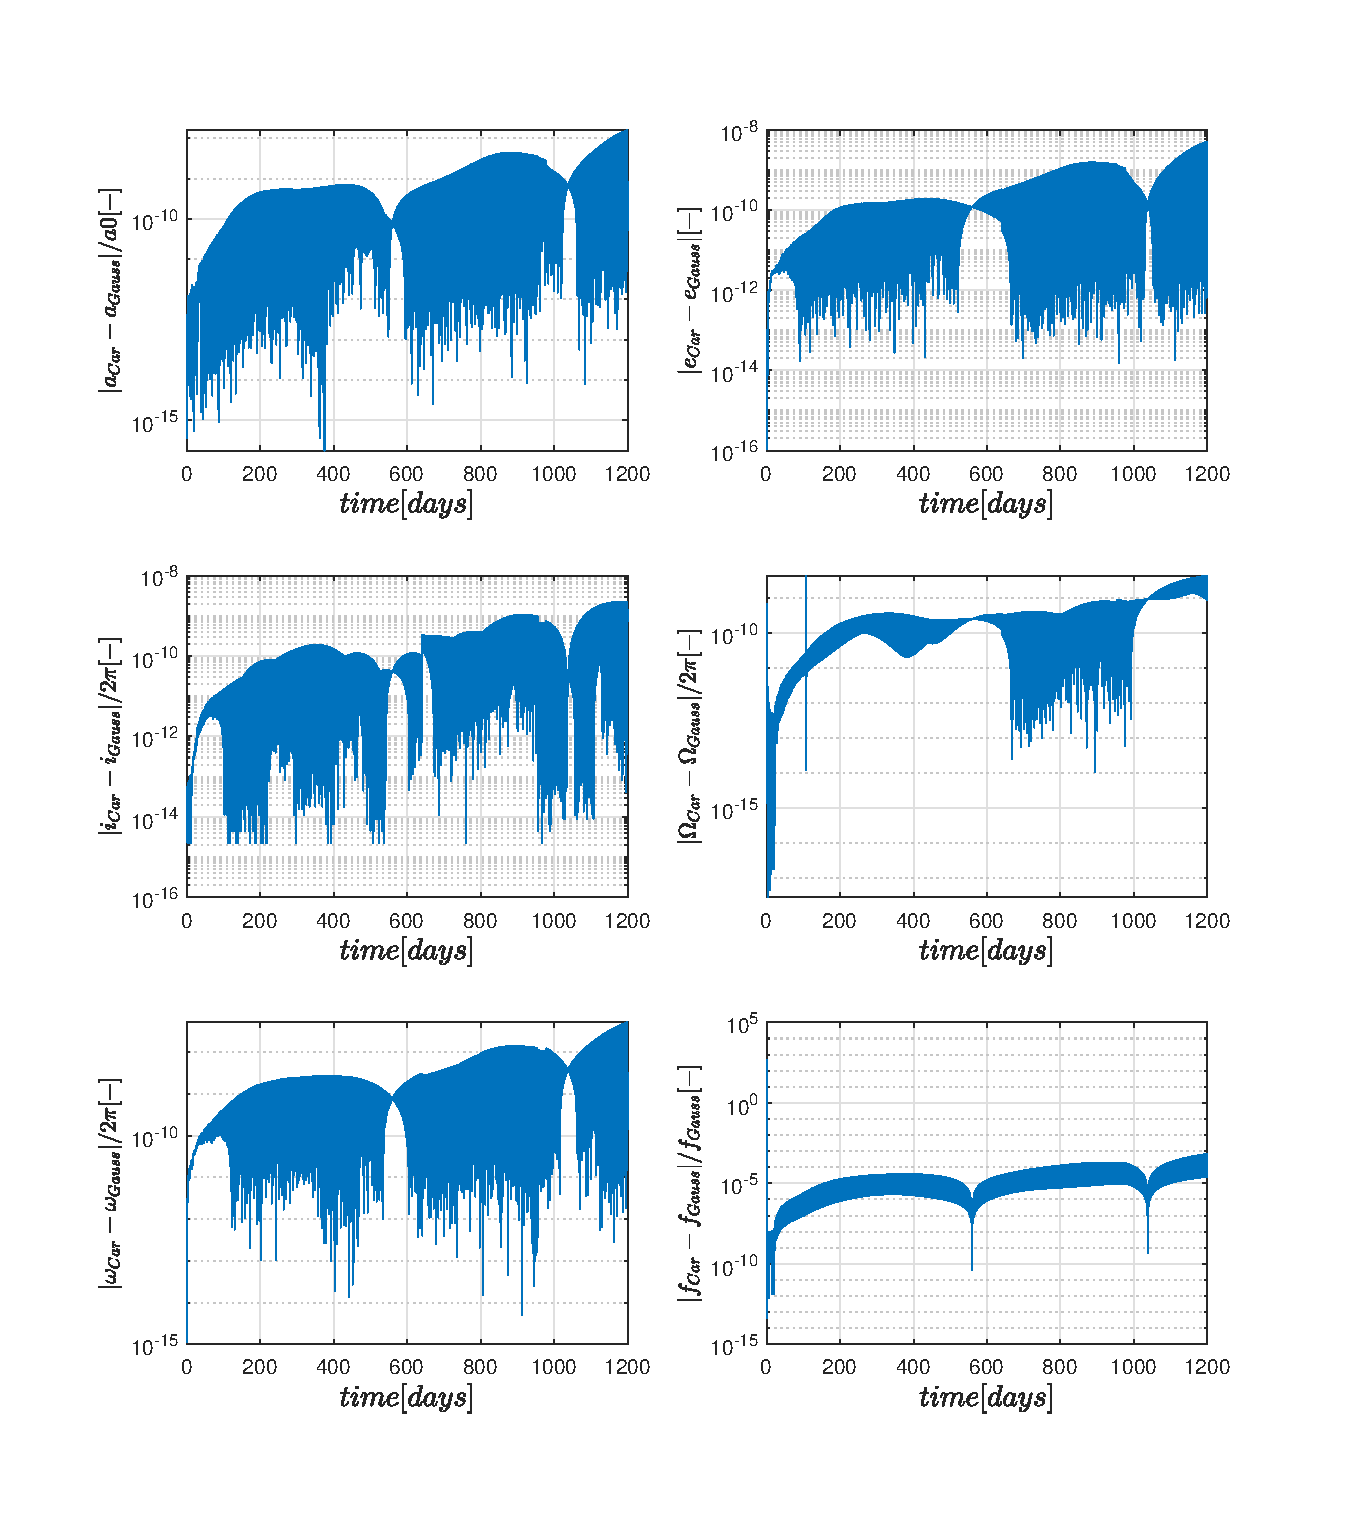
\epsfig{file= Perturbations/error.eps, width=\textwidth}
    \caption{error between Gaussian and Cartesian propagation methods (log scale)}
\end{figure}

\par
There are numerical error introducing differences between the two methods, but the error only grows up to an order between $10^{-10}$ and $10^{-8}$ for a propagation of 1200 days, except for the true anomaly which grows to a still small error of $10^{-3}$.


\section{History of the Keplerian elements}
% plot the history of every keplerian element
The Keplerian elements are plotted here for 1200 days from 2021-01-01
\begin{figure}[H]
\begin{tabular}{ccc}
\subfloat[semi-major axis]{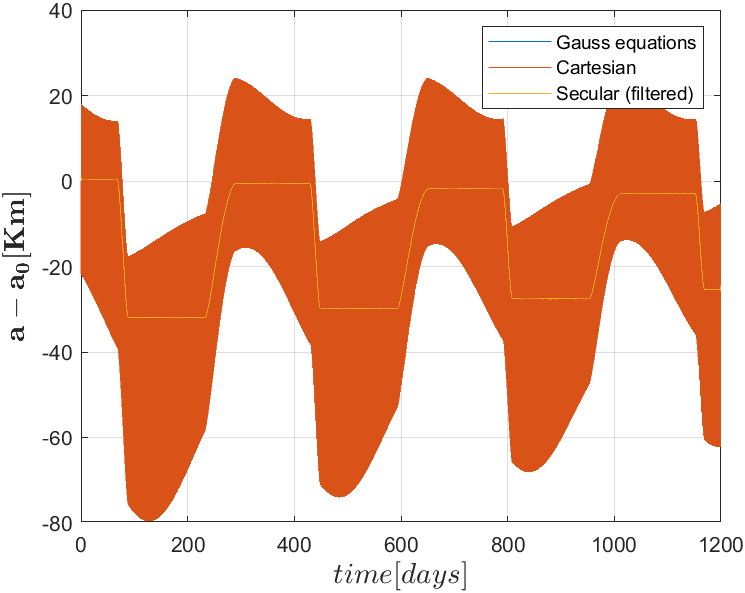
\includegraphics[width = 2.5in]{Perturbations/Evolution/a.png}} &
\subfloat[eccentricity]{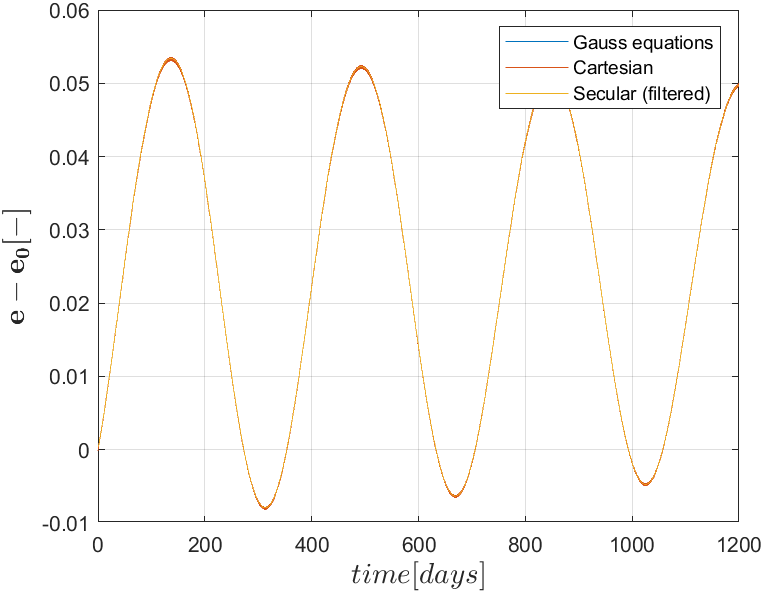
\includegraphics[width = 2.5in]{Perturbations/Evolution/e.png}} \\
\subfloat[inclination]{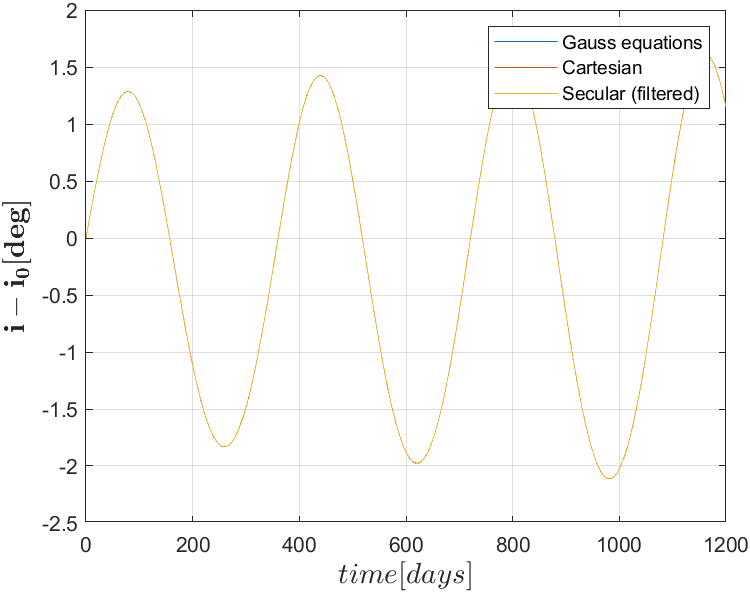
\includegraphics[width = 2.5in]{Perturbations/Evolution/i.png}} &
\subfloat[right ascension of ascending node]{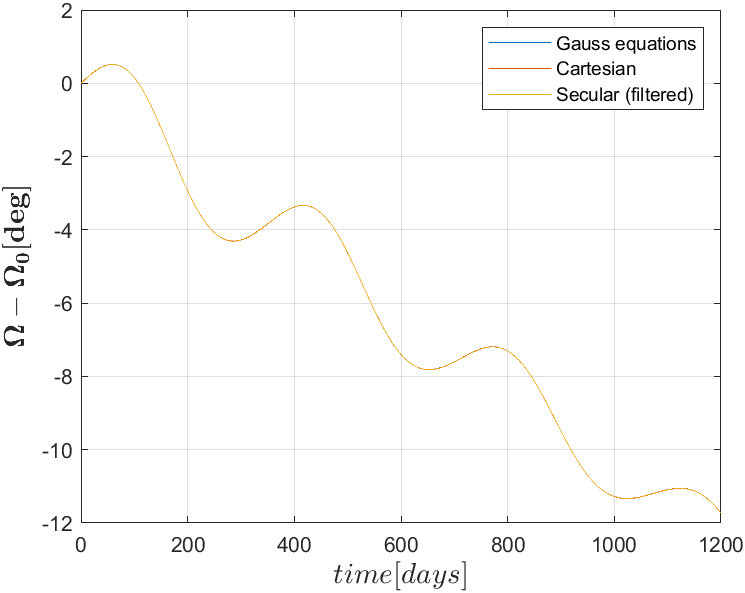
\includegraphics[width = 2.5in]{Perturbations/Evolution/RAAN.png}}\\
\subfloat[perigee anomaly]{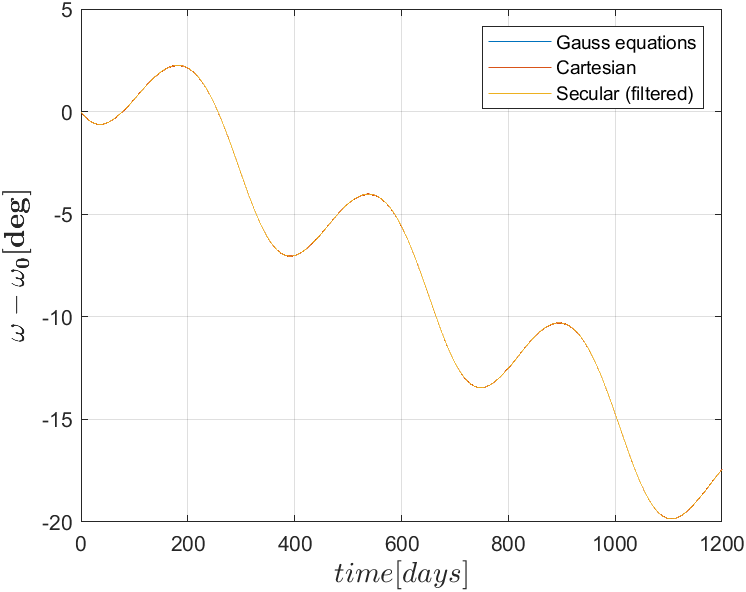
\includegraphics[width = 2.5in]{Perturbations/Evolution/omega.png}} &
\subfloat[true anomaly]{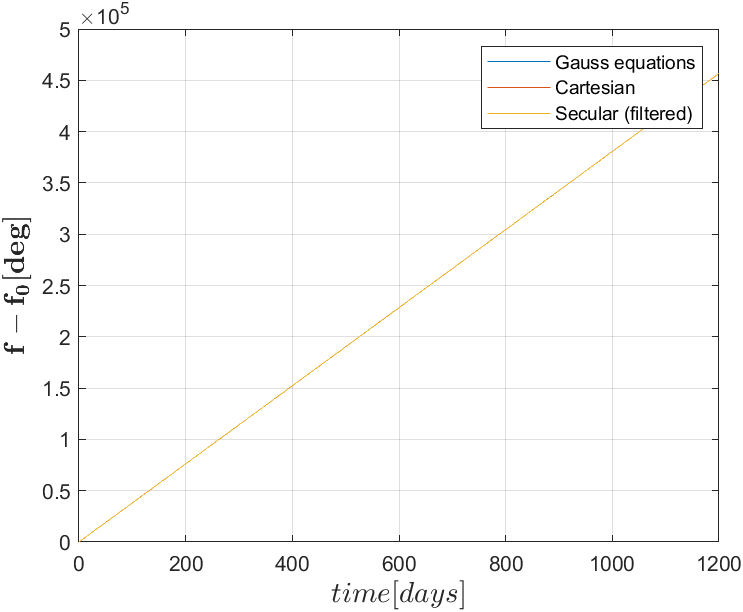
\includegraphics[width = 2.5in]{Perturbations/Evolution/f.png}} 
\end{tabular}

\caption{Evolution of keplerian elements}
\end{figure}

\section{Orbit evolution representation}

\section{HF filtering}
%Maybe we can do it when we plot the history of the Keplerian elements
For the filtering we have used the simple \emph{movmean} function integrated in MATLAB which computes the average at each time instant between the current point and the neighboring ones with a cutoff period of $3T_{orbit}$.

\par We can see in the \emph{secular evolution} that there is a superposition of effects from the J2 perturbation and the SRP:
\begin{itemize}
    \item \emph{$a$} : there is a slight secular decrease in the semi-major axis due to the effect of the SRP 
    \item \emph{$\Omega$} : there is a \emph{nodal regression} due to the inclination $i$ being less than $90\degree$ for the J2 effect
    \item  \emph{$\omega$} : there is a negative \emph{perigee precession} for the J2 effect due to the inclination $i\;> 63.4\degree$ giving a so-called \emph{"Hula-hooping effect"}
    \item \emph{$e$} : there are periodic oscillations with a secular increase caused by ovalization of the orbit by the SRP
\end{itemize}


\section{Comparison with real data}

\subsection{Satellite selection}

\subsection{Comparison with our model}

\begin{thebibliography}{9}
\bibitem{RSW_Curtis} 
Curtis, H.D. 
\textit{Orbital mechanics for engineering students}. 
Butterworth-Heinemann , 2014. Chapter 12

\bibitem{RSW_Vallado} 
Vallado, D.A.
\textit{Fundamental of Astrodynamics and Applications, 4th
Ed}, Microcosm Press, 2013. Chapters 8 and 9

\bibitem{RSW_Battin} 
Battin, R,
\textit{An Introduction to the Mathematics and Methods of
Astrodynamics}, AIAA Education Series, 1999. Chapter 10

\bibitem{SRP_Curtis} 
Curtis,H.D. 
\textit{Orbital mechanics for engineering students}. 
Butterworth-Heinemann , 2019. Chapter 10.9

\end{thebibliography}

\end{document}
